%!TEX root = ../thesis.tex
%*******************************************************************************
%*********************************** Background estimation *********
%*******************************************************************************


\chapter{Background estimation}

\ifpdf
    \graphicspath{{chapter-background/Figs/Raster/}{chapter-background/Figs/PDF/}{chapter-background/Figs/}}
\else
    \graphicspath{{chapter-background/Figs/Vector/}{chapter-background/Figs/}}
\fi

\glsreset{cr}

A reliable estimation of the expected \gls{sm} background rates in the \glspl{sr} is crucial for exercising the statistical machinery laid out in \cref{ch:statistics} and making conclusive statistical statements. The background estimation approaches used in the following either rely on semi-data-driven techniques or on \gls{mc}-only estimations. As estimating backgrounds only from \gls{mc} simulation is often problematic due to \eg mis-modelings in the phase space regions targeted not appropriately covered by the uncertainties, a (semi-)data-driven approach is often favoured. In the following, the major backgrounds $\ttbar$, single top and $\wjets$ are estimated using a semi-data-driven approach, while the expected rates from the remaining smaller backgrounds rely purely on \gls{mc} simulations and are normalised to their theoretical cross section.

\section{General strategy}

\subsection{Transfer factor approach}

Estimating background contributions in \glspl{sr} in a semi-data-driven approach, usually involves the introduction of so-called \glspl{cr} used to control dominant background processes by comparing their expected event rates to data. The \glspl{cr} are designed to be enriched in events of a given background process (or type) while being approximately free of signal contamination. If $N_p^\mathrm{MC}(\mathrm{SR})$ and $N_p^\mathrm{MC}(\mathrm{CR})$ are the expected rates for a given background process $p$ from \gls{mc} simulation in a given \gls{sr} and \gls{cr}, respectively, then the transfer factor $N_p^\mathrm{MC}(\mathrm{SR})/N_p^\mathrm{MC}(\mathrm{CR})$ allows to convert the number of observed background events in the \glspl{cr}, $N_p^\mathrm{obs.}(\mathrm{CR})$ into a background estimate in the \glspl{sr},$N_p^\mathrm{est.}(\mathrm{SR})$, through
\begin{equation}
	N_p^\mathrm{est.}(\mathrm{SR}) = N_p^\mathrm{obs.}(\mathrm{CR}) \frac{N_p^\mathrm{MC}(\mathrm{SR})}{N_p^\mathrm{MC}(\mathrm{CR})} = \mu_p N_p^\mathrm{MC}(\mathrm{SR}).
	\label{eq:transfer_factor}
\end{equation}
An important benefit of this approach is that the impact of systematic uncertainties on the estimated background rates can be evaluated on the transfer factors, that are ratios of \gls{mc} estimates. As such, systematic uncertainties can be canceled in the extrapolation to the \gls{sr}. The uncertainty on the background estimate is then a combination of statistical uncertainties in the \gls{cr} and remaining uncertainties affecting the extrapolation. For this reason, \glspl{cr} are usually deliberately chosen to have large statistics, effectively reducing the uncertainties on the extrapolation to the \glspl{sr}.  

As indicated in~\cref{eq:transfer_factor}, the transfer factor approach is formally equivalent to using the process-specific normalisation factor introduced in~\cref{sec:likelihood_function}, effectively \textit{normalising} the number of background events expected from \gls{mc} in the \gls{cr} to the number of observed events. In the profile likelihood fit setups used in the following, implemented using \textsc{HistFitter}~\cite{HistFitter:2014wma}, the normalisation factor $\mu_b$ is fitted to data instead of background as expected from \gls{mc} simulation. In the following, multiple disjoint \glspl{cr} are used to simultaneously normalise multiple background processes to data in a combined fit. In order not to have an underdetermined minimisation problem, at least the same number of \glspl{cr} as normalisation factors needs to be used. Two different profile likelihood fit configurations are used in the following, a \textit{background-only} fit configuration assuming no signal contribution and typically only including the \glspl{cr}, and a \textit{model-dependent} fit configuration with nominal signal contribution using \glspl{cr} as well as \gls{sr}.

In order to verify the quality of the extrapolation from the \glspl{cr} to the \glspl{sr}, so-called \gls{vr} are defined. \glspl{vr} do not participate in the actual fit of the model parameters to data, but serve as intermediate regions to verify the extrapolation. For this reason, \glspl{vr} are typically placed in the region between the \glspl{cr} and \glspl{sr} that is extrapolated over. A schematic view of an analysis strategy using all three types of regions is shown in~\cref{fig:hf_strategy}. All three types of regions can have more than one bin and are separated using suitable observables that are extrapolated over.


\begin{figure}
\floatbox[{\capbeside\thisfloatsetup{capbesideposition={right,center},capbesidewidth=0.5\textwidth}}]{figure}[\FBwidth]
{\caption{Schematic view of an analysis strategy including multiple control, validation and signal regions with one or multiple bins each. Extrapolations from the control regions into the signal regions can be verified in the validation regions lying in the phase space extrapolated over. Figure adapted from~\cite{HistFitter:2014wma}.}\label{fig:hf_strategy}}
{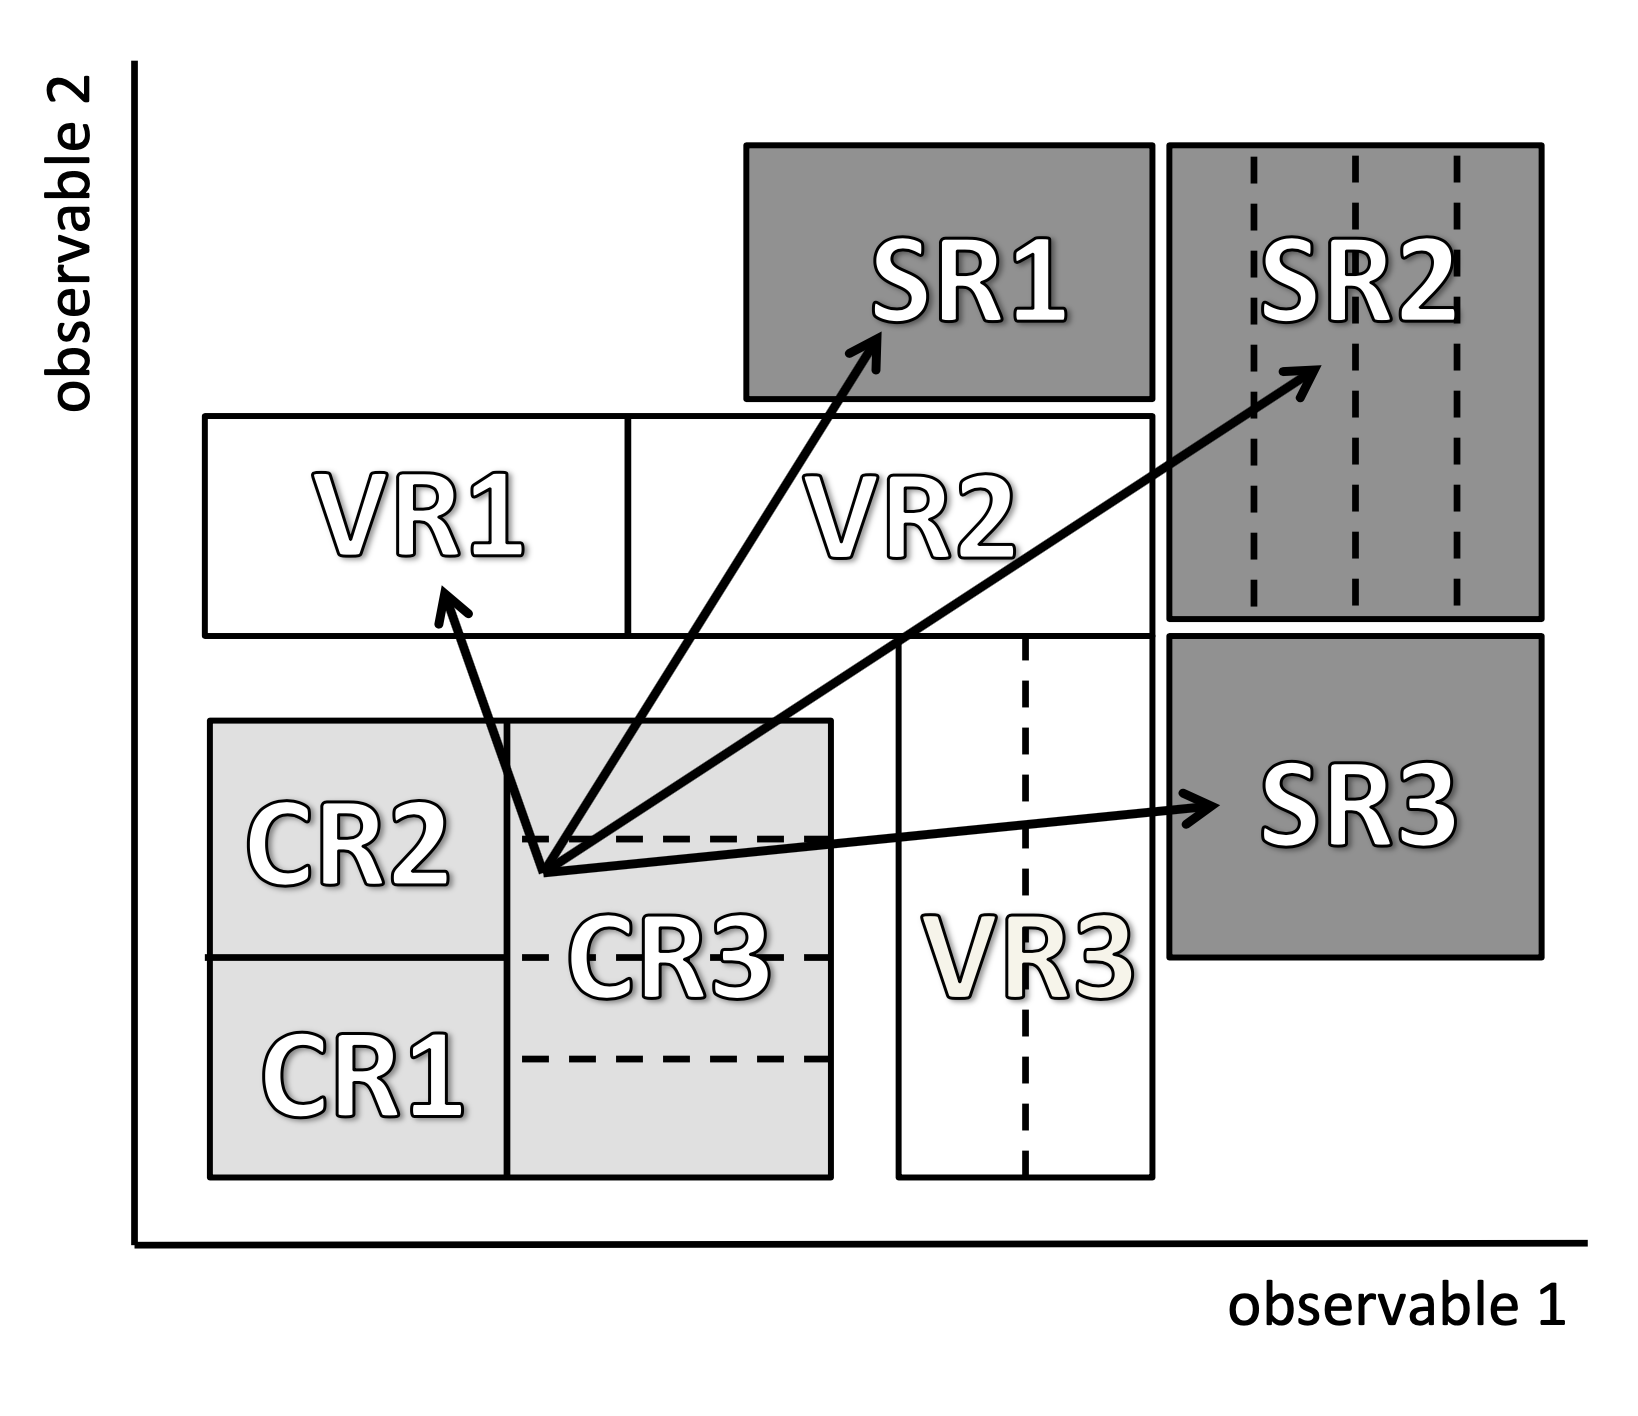
\includegraphics[width=0.45\textwidth]{hf_strategy}}
\end{figure}


\subsection{Analysis blinding}

An important concept in the design phase of searches for new physics is the idea of \textit{blinding} regions of interest~\cite{blind:2003rw}, meaning that measured data are not looked at in these regions. This avoids issues of \textit{experimenter's bias}, \ie unintended influences on the design of the analysis based on the observed data. If data were already known when designing the signal regions (and therefore the outcome of the analysis would be known to some extent), experimenter's bias could for example occur during the selection of the final signal region definitions.

During the design of a search for new physics, signal regions are generally kept blinded until the complete analysis strategy is fixed. Once the \glspl{sr} have been designed, the next step is to develop suitable \glspl{cr} with negligible signal contamination. This is followed by design of \glspl{vr} that can be unblinded once the \glspl{cr} are fixed. The \glspl{sr} are only unblinded after the extrapolation from the \glspl{cr} has been verified in the \glspl{vr}, allowing to either quantify potential excesses in data or set limits on model parameters. 

\section{Control regions}

The contributions from $\ttbar$, $\wjets$ production and single top processes are normalised to data in dedicated \glspl{cr}. All \glspl{cr} are designed to be kinematically as close as possible to the respective \glspl{sr}, such that the normalisation factors derived in the \glspl{cr} are also valid in the \glspl{sr}. The \glspl{cr} are mutually exclusive and made orthogonal to the \glspl{sr} through their requirements on $\mt$, $\mct$ and $\mbb$. \Cref{fig:cr_strategy} illustrates the configuration of all \glspl{cr}, especially highlighting the fact that all \glspl{cr} are located in sideband regions off the $\mbb$ window, significantly reducing signal contamination.

Subdominant processes like $\zjets$, diboson and multiboson, $\ttbar+V$, $\ttbar+h$ and $V+h$ are estimated directly from \gls{mc} simulation and normalised to their theoretical cross sections. 

\subsubsection[Control regions for $\ttbar$]{Control regions for $\boldsymbol{\ttbar}$}



\subsubsection{Control region for single top}

\subsubsection[Control region for $\wjets$]{Control regions for $\boldsymbol{\wjets}$}


\begin{table}
\begin{center}
\resizebox{\textwidth}{!}{
\begin{tabular} {l | c c c | cccccc}
\toprule
\textbf{CR} & \textbf{TR-LM} &  \textbf{TR-MM} &  \textbf{TR-HM} &  \multicolumn{3}{c}{\textbf{WR}} & \multicolumn{3}{c}{ \textbf{STR}} \\                 
\midrule
$\mbb$ [$\GeV$]  & \multicolumn{3}{c|}{$<$100 or $>$140} & \multicolumn{3}{c}{$\in[50,80]$} &\multicolumn{3}{c}{$>$195}\\
$\mt$ [$\GeV$]   & $\in[100,160]$ & $\in[160,240]$ & $>$240 & \multicolumn{3}{c}{$\in[50,100]$} &\multicolumn{3}{c}{$>$100}\\
$\mct$ [$\GeV$]  &\multicolumn{3}{c|}{$<$180} & \multicolumn{3}{c}{$>$180} &\multicolumn{3}{c}{$>$180}\\
\midrule
\textbf{VR} & \textbf{VR-onLM} &  \textbf{VR-onMM} & \textbf{VR-onHM} & \multicolumn{2}{c}{ \textbf{VR-offLM}} &  \multicolumn{2}{c}{\textbf{VR-offMM}} &  \multicolumn{2}{c}{\textbf{VR-offHM}}\\
\midrule
$\mbb$ [$\GeV$]  & \multicolumn{3}{c|}{$\in[100,140]$} & \multicolumn{2}{c}{$\in[50,80]\, \cup [160, 195]$} & \multicolumn{2}{c}{$\in[50,80]\, \cup [160, 195]$}& \multicolumn{2}{c}{$\in[50,75]\, \cup [165, 195]$}\\
$\mt$ [$\GeV$]   & $\in[100,160]$ & $\in[160,240]$ & $>$240 & \multicolumn{2}{c}{$\in[100,160]$} & \multicolumn{2}{c}{$\in[160,240]$} & \multicolumn{2}{c}{$>$240}\\
$\mct$ [$\GeV$]  &\multicolumn{3}{c|}{$<$180}&\multicolumn{6}{c}{$>$180}\\
\bottomrule
\end{tabular}}
\caption{Overview of the CR and VR definitions. All regions partially share the same selection as the SR for all variables except $\mlb$, which is not used in the CR and VR definitions.} 
\label{tab:CRVRdef}
\end{center}
\end{table}



\begin{figure}
\floatbox[{\capbeside\thisfloatsetup{capbesideposition={right,center},capbesidewidth=0.5\textwidth}}]{figure}[\FBwidth]
{\caption{Configuration of the control regions, placed around the signal regions off the $\mbb$ window.}\label{fig:cr_strategy}}
{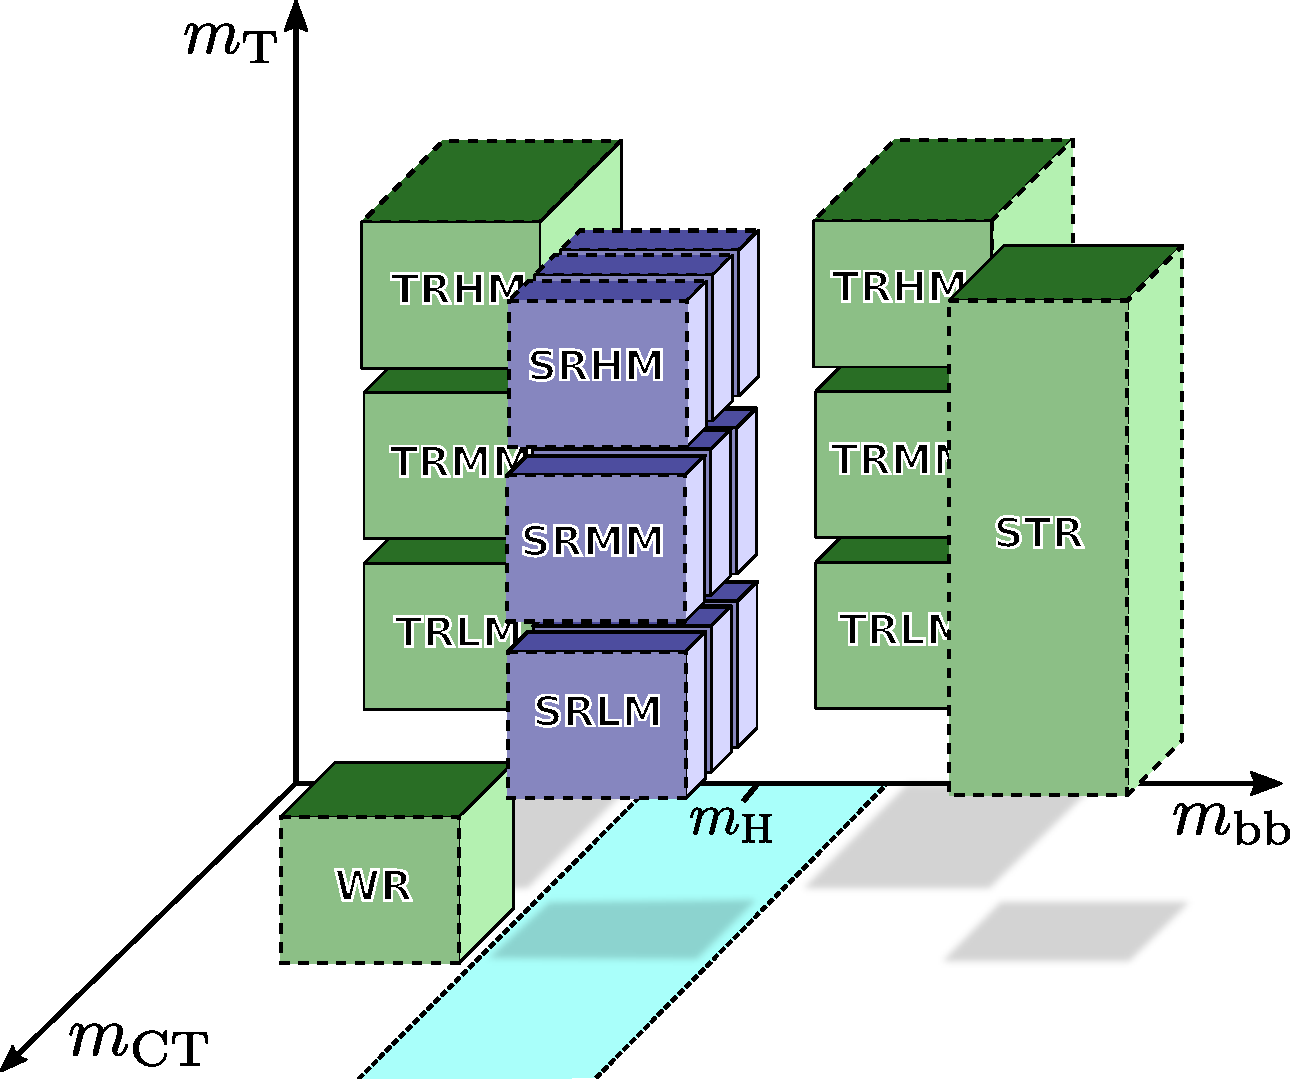
\includegraphics[width=0.45\textwidth]{strategy_5}}
\end{figure}

\section{Validation regions}



\begin{figure}
\floatbox[{\capbeside\thisfloatsetup{capbesideposition={right,center},capbesidewidth=0.5\textwidth}}]{figure}[\FBwidth]
{\caption{Configuration of the validation regions in the phase space between the \glspl{cr} and \glspl{sr}. The \glspl{vr} are arranged such that each of the three extrapolation dimensions can be validated.}\label{fig:vr_strategy}}
{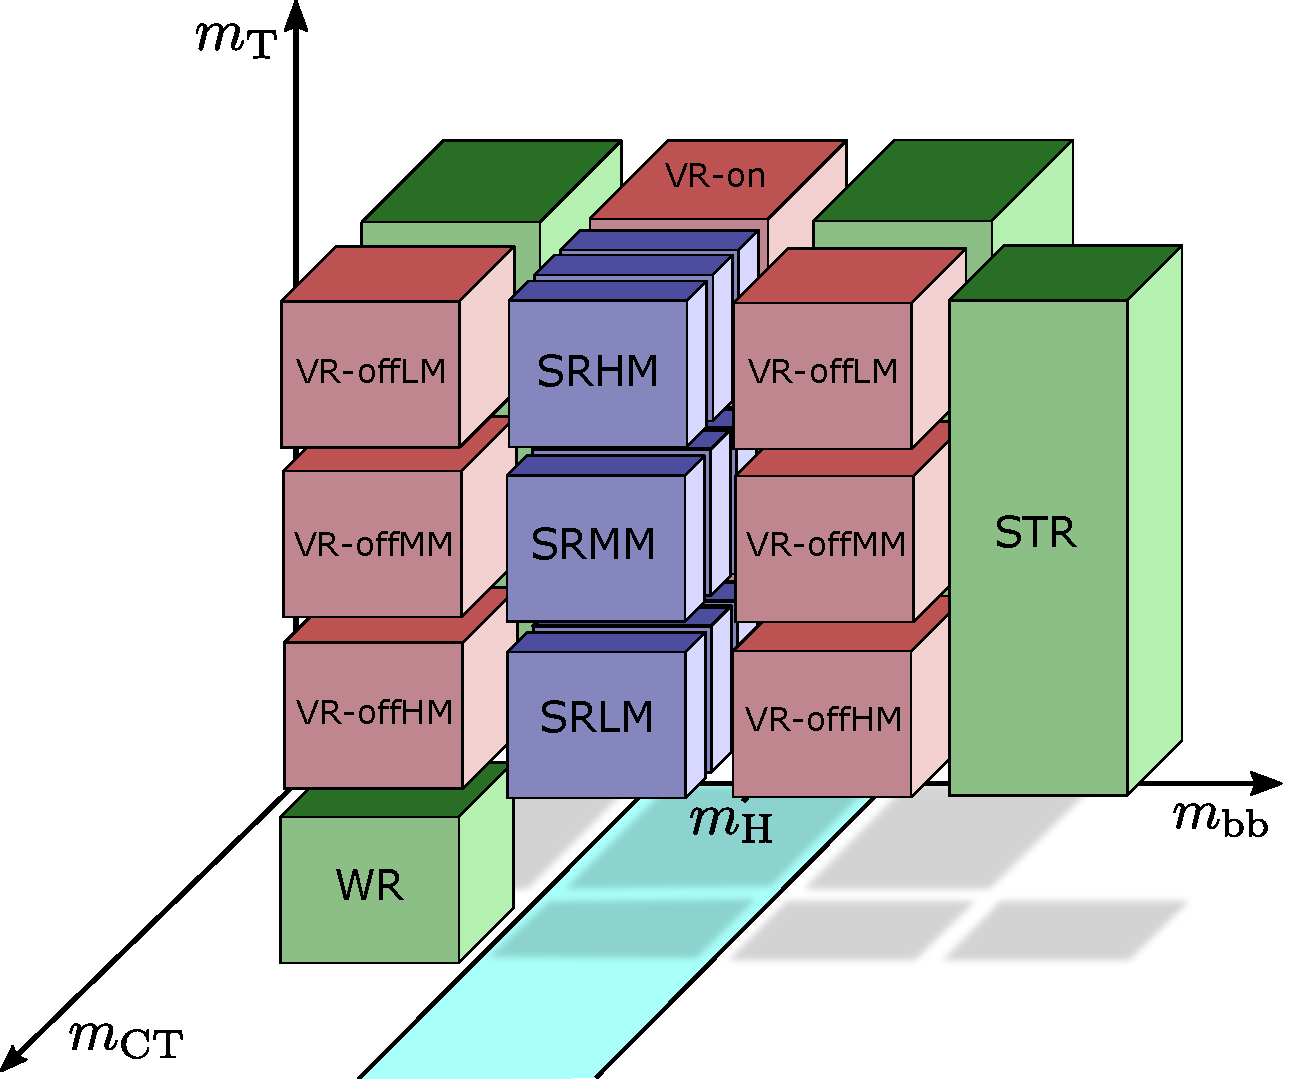
\includegraphics[width=0.45\textwidth]{strategy_7}}
\end{figure}
